\section{Aula 07}
    \subsection{Exercício 5}
        \begin{figure}[H]
            \centering
            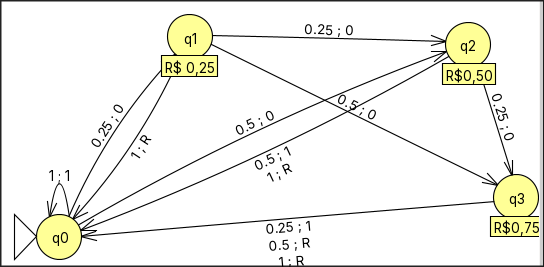
\includegraphics[width=0.8\textwidth]{Aula07/Images/Exercicio1.png}
            \caption*{1}
        \end{figure}
        Diagrama de Estados:
        \begin{itemize}
            \item q0 (estado inicial)
                \begin{itemize}
                    \item $0.25 \to q1 | S = 0$
                    \item $0.50 \to q2 | S = 0$
                    \item $1.00 \to q0 | S = 1$
                \end{itemize}
            \item q1
                \begin{itemize}
                    \item $0.25 \to q2 | S = 0$
                    \item $0.50 \to q0 | S = 1$
                    \item $1.00 \to q0 | S = R$
                \end{itemize}
            \item q2
                \begin{itemize}
                    \item $0.25 \to q3 | S = 0$
                    \item $0.50 \to q0 | S = 1$
                    \item $1.00 \to q0 | S = R$
                \end{itemize}
            \item q3
                \begin{itemize}
                    \item $0.25 \to q0 | S = 1$
                    \item $0.50 \to q0 | S = R$
                    \item $1.00 \to q0 | S = R$
                \end{itemize}                
        \end{itemize}
    
    \subsection{Exercício 6}
        \begin{figure}[H]
            \centering
            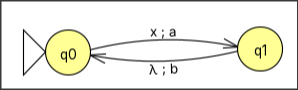
\includegraphics[width=0.8\textwidth]{Aula07/Images/Exercicio2.png}
            \caption*{1}
        \end{figure}

        \[AF = (\{Parado, Subindo, Descendo\}, \{=, >, <\}, \{P, S, D\}, \delta, \gamma, q0)\]
        
        \begin{itemize}
            \item Função de transição ($\delta$):
                \begin{center}
                    \begin{tabular}{|c|c|c|}
                        \hline
                        Estado Atual & Condição & Próximo Estado | Saída \\
                        \hline
                        $q_0$ & requisitado $=$ atual & $q_0 \,|\, S = Parar$ \\
                        \hline
                        $q_1$ & requisitado $=$ atual & $q_0 \,|\, S = Parar$ \\
                        \hline  
                    \end{tabular}
                \end{center}
                
            \item Função Saída ($\gamma$):
            \begin{center}
                \begin{tabular}{|c|c|c|}
                    \hline
                    Estado Atual & Entrada & Saída\\
                    \hline
                    $q_0$ & $x$ & $a$\\
                    \hline
                    $q_1$ & Subir\\
                    \hline
                    Descendo & Descer\\
                    \hline
                \end{tabular}
            \end{center}
        \end{itemize}

        Diagrama de Estados:
        \begin{itemize}
            \item q0 (estado inicial)
                \begin{itemize}
                    \item $x \to q1 | S = a$
                \end{itemize}
            \item q1
                \begin{itemize}
                    \item $\lambda \to q0 | S = b$
                \end{itemize}
        \end{itemize}

    \subsection{Exercício 7}
        \begin{figure}[H]
            \centering
            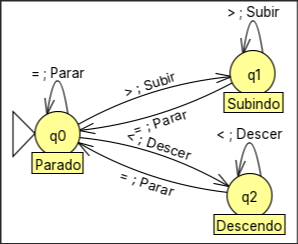
\includegraphics[width=0.8\textwidth]{Aula07/Images/Exercicio7.png}
            \caption*{7}
        \end{figure}
        
        \[AF = (\{Parado, Subindo, Descendo\}, \{=, >, <\}, \{P, S, D\}, \delta, \gamma, q0)\]
        
        \begin{itemize}
            \item Função de transição ($\delta$):
                \begin{center}
                    \begin{tabular}{|c|c|c|}
                        \hline
                        Estado Atual & Condição & Próximo Estado | Saída \\
                        \hline
                        $q_0$ & requisitado $=$ atual & $q_0 \,|\, S = P$ \\
                        $q_0$ & requisitado $>$ atual & $q_1 \,|\, S = S$ \\
                        $q_0$ & requisitado $<$ atual & $q_2 \,|\, S = D$ \\
                        \hline
                        $q_1$ & requisitado $=$ atual & $q_0 \,|\, S = P$ \\
                        $q_1$ & requisitado $>$ atual & $q_1 \,|\, S = S$ \\
                        \hline
                        $q_2$ & requisitado $=$ atual & $q_0 \,|\, S = P$ \\
                        $q_2$ & requisitado $<$ atual & $q_2 \,|\, S = D$ \\
                        \hline  
                    \end{tabular}
                \end{center}
                
            \item Função Saída ($\gamma$):
            \begin{center}
                \begin{tabular}{|c|c|}
                    \hline
                    Parado & Parar\\
                    \hline
                    Subindo & Subir\\
                    \hline
                    Descendo & Descer\\
                    \hline
                \end{tabular}
            \end{center}
        \end{itemize}
